% Please use the skeleton file you have received in the
% invitation-to-submit email, where your data are already
% filled in. Otherwise please make sure you insert your
% data according to the instructions in PoSauthmanual.pdf
\documentclass{PoS}

\usepackage{siunitx}
\usepackage{caption}
\usepackage{subcaption}

\newcommand{\micron}{\si{\micro\meter}}
% \DeclareCaptionSubType*[arabic]{figure}
\renewcommand{\subfigurename}{Fig.}
\renewcommand{\thesubfigure}{\thefigure.\alph{subfigure}}
\captionsetup[subfigure]{font=scriptsize,labelformat=simple,labelsep=colon}

\title{Pixel Telescope to test pixel Phase II ROCs and sensors}

\ShortTitle{Telescope to Test CMS Upgrade Pixel Detectors}

\author{\speaker{Caleb Fangmeier}\\
  Univ.\ of Nebraska \-- Lincoln\\
  E-mail: \email{cfangmei@cern.ch}}

%\author{Another Author\\
%        Affiliation\\
%        E-mail: \email{...}}

\abstract{\
A silicon-strip sensor based particle telescope is being developed to
aid in the characterization of next-generation silicon-pixel detectors for
the Compact Muon Solenoid (CMS) detector at the Large Hadron Collider (LHC).
This telescope is expected to enable sub-micron feature studies of prototype
detectors by combining 25-{\micron} pitch strip detectors with a very low noise
readout system. Additionally, this telescope improves upon previous iterations
by deploying a parallel readout scheme to increase the maximum trigger rate by
a factor of 16.
}

\FullConference{38th International Conference on High Energy Physics\\
    3-10 August 2016\\
    Chicago, USA}

\begin{document}

\section{Introduction}

The innermost element of the CMS detector at the LHC is the silicon pixel
tracker. The current version of the tracker has performed well and been
critical to the physics program of CMS. The High Luminosity LHC upgrade of CMS
will replace the entire silicon tracking system.  As part of this upgrade, a
new section of the pixel tracker is proposed to be added in the so-called
``very-forward'' ($\eta\sim4$) region of the detector. Because the particles in
this region are traveling almost parallel to the magnetic field of the
detector, enhanced $\phi$ sensitivity is required to accurately measure track
curvature, a critical measurement for finding particle momentum and charge.
The proposed new detector section will feature pixels with increased elongation,
relative to the current CMS pixel tracker, for enhanced $\phi$ sensitivity,
while sacrificing sensitivity in $\rho$.  This contribution presents a
telescope being developed primarily to characterize these elongated pixel
geometries.

The telescope consists of eight layers of silicon-strip sensors, with the
prototype pixel detector placed in the center surrounded by four strip sensor
layers on either side. A beam of charged particles is directed to pass through
both the strip sensors and the prototype pixel sensors.  Measurements from the
telescope are taken to reconstruct individual particle tracks. These tracks are
then compared to data collected from the pixel sensor to characterize its
performance.

\section{Hardware}
The telescope has been designed around a specific silicon-strip sensor and
accompanying readout chip, both of which were originally developed for the H1
vertex detector at HERA~\cite{Hilgers2001}. The strip sensor contains 512
strips with $25\micron$ pitch. The readout chip is the
``Analog~Pipeline~Chip~\--~128'' (APC).  Each APC can read 128 strips so four
chips are required to read a single strip sensor. The APC operates an
integrating pre-amplifier that collects charge from a single sensor strip and
keeps a 32-sample history of the output of that pre-amplifier. When a trigger
is received from, for example, a scintillation detector indicating a particle
has passed through the telescope, the appropriate sample is chosen from the
32-sample history based on the calibrated trigger latency and the selected
samples from all 128 channels of the APC are serialized to its output.

\begin{figure}[h]
  \centering
  \begin{subfigure}[t]{0.45\textwidth}
    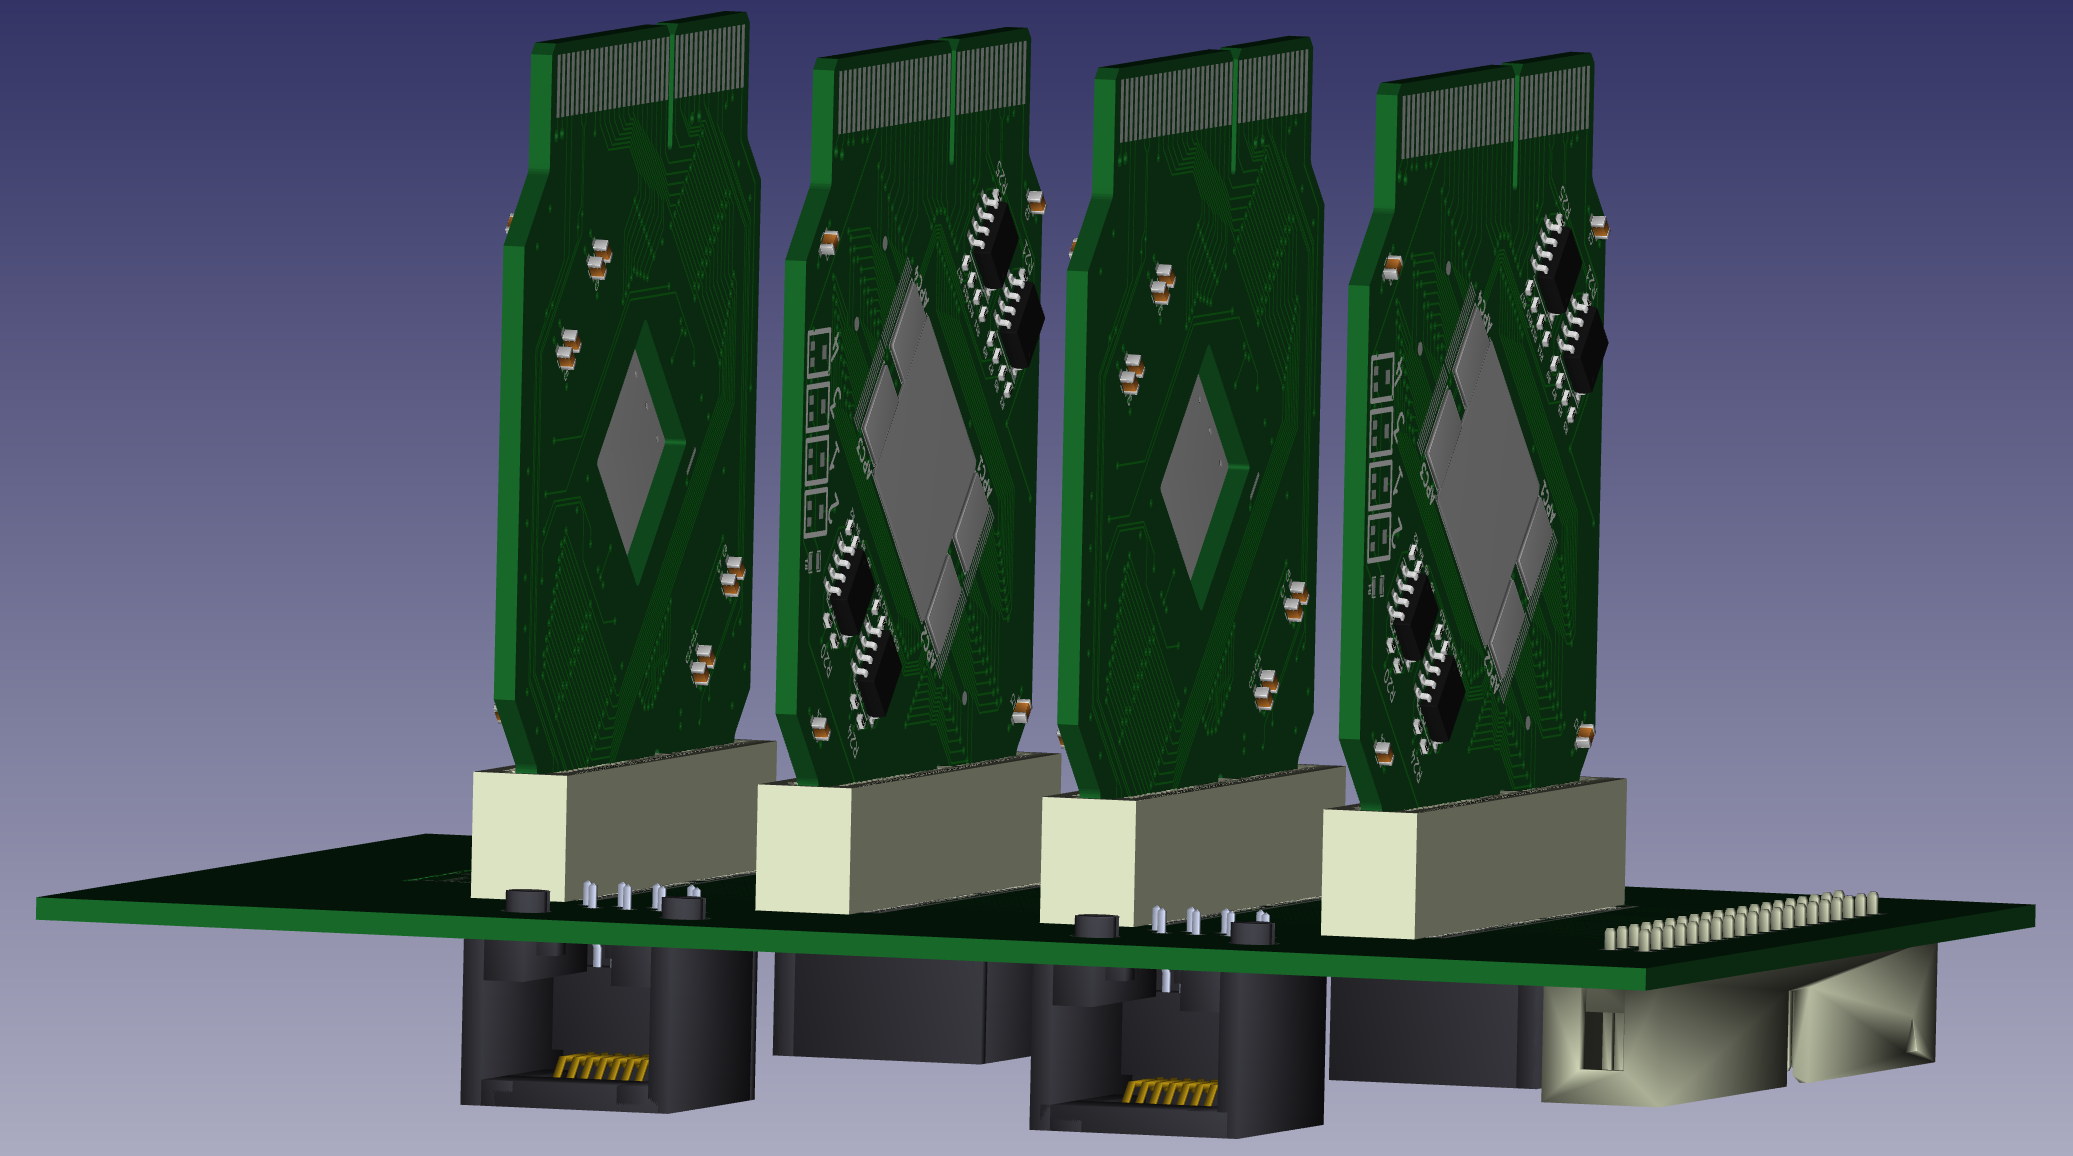
\includegraphics[width=\textwidth]{../figures/Half-Telescope-Full.png}
    \caption{A rendering of the telescope ``motherboard'' showing four
      ``sensor-cards'' each of which holds a single strip sensor. The control
      signals needed by the readout chip are supplied by a 40-pin header
      (bottom-right). The data readout happens over four RJ-45 connectors (bottom-center), into
      which CAT-5 cables are plugged to transmit the signals to the DAQ board.}
\label{fig:hardware:motherboard}
  \end{subfigure}
  \hspace{.3in}
  \begin{subfigure}[t]{0.45\textwidth}
    \includegraphics[width=\textwidth]{../figures/DAQ_Board_Real.png}
    \caption{An image of the DAQ board featuring an $8\times$RJ-45
      connector (back) to receive data from two connected motherboards, a
      $2\times40$-pin header (front) for supplying control signals to the
      motherboards, and an Opal-Kelly FPGA integration module (center) to
      orchestrate the operation of the telescope.}
\label{fig:hardware:daq}
  \end{subfigure}
  % \caption{The main hardware components of the telescope are the motherboard
  %   with associated sensor-cards (a) and the data acquisition board (b)}
\label{fig:hardware}
\end{figure}

The strip sensor and four APC are mounted onto a sensor-card along
with four buffer amplifiers that compensate for the relatively weak output of
the APC and generate a more robust differential signal with the proper output
impedance for driving CAT-5 cables ($100\si{\ohm}$). Four sensor-cards are
plugged into a motherboard (Fig.~\subref{fig:hardware:motherboard}) which provides mechanical support for the
sensor-cards and routes electrical signals between the sensor cards and the I/O
ports.

The signals from the two motherboards that constitute the telescope are routed
to the data acquisition (DAQ) board (Fig.~\subref{fig:hardware:daq}). The DAQ board contains eight
40\si{\mega\hertz} 10-bit ADCs with four channels each, giving a total of 32
digitization channels. The DAQ board also contains circuitry for supplying the
bias voltage for the strip detectors, and LEMO connectors for supplying an
external trigger and clock signal. Digital logic is implemented via an Opal
Kelly FPGA integration module which features an Altera Cyclone IV FPGA, 128MB
of RAM, and a Super-Speed USB link for data transfer.

\section{Readout Scheme}
The readout scheme has been designed to minimize the time required to transfer
the strip sensor pulse-height values from the APC to the DAQ board.  The APC
cannot record data during readout so increasing the data transfer speed results
in a reduction of dead time.  As illustrated in Fig.~\ref{fig:readout}, the
readout happens in three stages.

The first stage is handled by the electronics
in and near the beam. It is here that the ionization caused by the passage of a
charged particle is converted to an electronic pulse by the strip sensor and
the height of that pulse is recorded by the APC. The APC then serializes pulse
heights from many strips to the cables exiting the beam region.

In the second stage, signals from the telescope are received by the DAQ
board where they are digitized and fed into an FPGA. The FPGA contains firmware
that is responsible for dropping strip readings with pulse-heights below a
set threshold and grouping the remaining strips into ``hit'' objects. These hit
objects, along with their associated trigger id, are then pushed to a connected
PC via a USB link.

The third stage consists of software that receives the hit data from the DAQ
board, constructs events from them, and saves the events to disk.
Offline analysis software then uses this data to identify the individual tracks
of particles passing through the telescope. Detector alignment studies will
also be critical to measuring the position of the strip sensors to micron
precision. Finally, the tracks can be interpolated to the impact point with the
prototype pixel detector and used to measure its properties.
\begin{figure}[h]
  \centering
  \begin{subfigure}[b]{0.49\textwidth}
    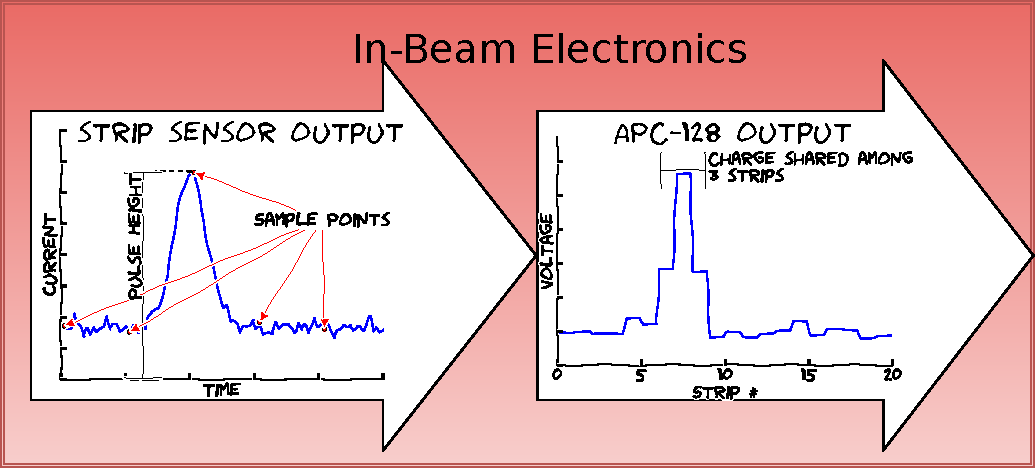
\includegraphics[height=1.32in]{../figures/Telescope_Data_Flow_Stage_I.pdf}
  \end{subfigure}
  \begin{subfigure}[b]{0.49\textwidth}
    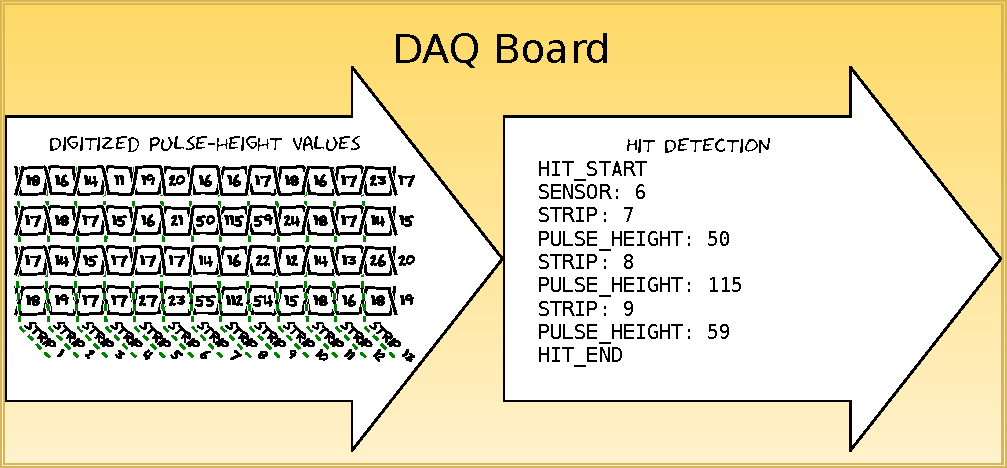
\includegraphics[height=1.32in]{../figures/Telescope_Data_Flow_Stage_II.pdf}
  \end{subfigure}
  \begin{subfigure}[b]{0.49\textwidth}
    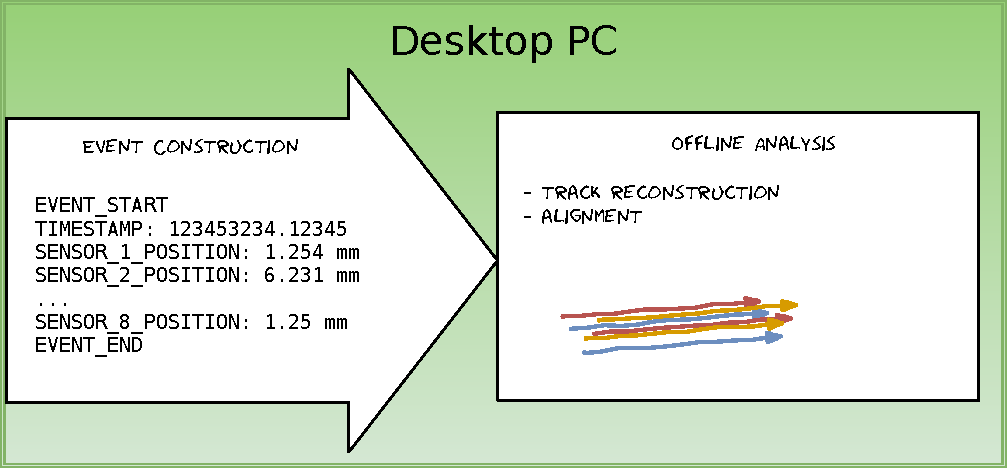
\includegraphics[height=1.32in]{../figures/Telescope_Data_Flow_Stage_III.pdf}
  \end{subfigure}
  \caption{Illustration of the readout scheme of the telescope.}
\label{fig:readout}
\end{figure}


\section{Projected Telescope Performance}
The performance of the telescope can be quantified in two ways: the
precision with which individual particle trajectories can be measured, and
the rate at which data can be collected.

The measurement precision of particle tracks depends on the number of detector
layers and the single layer spatial resolution. The telescope consists of eight
silicon-strip sensor layers with $25\micron$ pitch. For strip sensors
with charge sharing the single hit precision can be approximated by the
pitch divided by the signal-to-noise ratio of the readout system.
The expected signal-to-noise ratio of the telescope is 25~\cite{Ryser2013}. This yields a single-hit precision of
$\approx1\micron$. This single-hit precision combined with two measurements in
each dimension on each side of the prototype sensor should give sub-micron
track localization at the point of impact with the prototype sensor.

Because many test-beam facilities have beam rates on the order of
\si{\mega\hertz}, only a small fraction of time during data taking will be
spent waiting for a trigger. Therefore, increasing the telescope's maximum
trigger rate will significantly increase the amount of data that can be
collected during a test beam.  Furthermore, the trigger rate for the telescope
is primarily limited by the time required to transfer 128 pulse-height values
from the APC to the DAQ Board.  A previous version of this telescope used the
daisy-chain feature of the APC to serialize the readout of 16 APC into a single
readout channel\cite{Turner2012}. This simplified the DAQ because it reduced the number of
digitization channels from 32 to 2, but also increased the readout time by a
factor of 16. The new version of the telescope will avoid this performance
penalty by reading out all 32 APC in parallel. In addition to parallel readout, the
trigger rate can be improved by optimizing the readout electronics using well
established RF design techniques. For example, placing buffer amplifiers near
the APC will reduce the rise-time of signals as they propagate along the cables
to the DAQ board, while using differential signaling on these same cables will
reduce electro-magnetic interference from the environment. With these
improvements a maximum trigger rate of $\approx15\si{\kilo\hertz}$ is expected.


\begin{thebibliography}{99}
  \bibitem{Hilgers2001}
M. Hilgers,
\emph{Development of a radiation hard version of the Analog Pipeline Chip APC128},
\emph{Nucl. Instrum. Meth.} A481:556-565,2002
[{\tt hep-ex/0101023}].
  \bibitem{Ryser2013}
A. Ryser,
\emph{Semesterarbeit \-- Pixel Telescope},
2013, unpublished.
  \bibitem{Turner2012}
P. Turner,
\emph{Design and Implementation of a High Resolution Telescope for CMS Pixel Detector Characterization},
2012, unpublished.
\end{thebibliography}

\end{document}
